\documentclass[11pt,english]{article} % Idioma
\usepackage[T1]{fontenc}
\usepackage{textcomp, verbatim} % \begin{comment}
\usepackage[utf8]{inputenc} % Permite acentos

\usepackage{wrapfig} % Imagenes %\graphicspath{ {./imagenes/} }
\usepackage[left=2.75cm,top=2.5cm,right=2cm,bottom=2.5cm]{geometry} % Márgenes
\usepackage{amssymb, amsmath, amscd, amsfonts, amsthm, mathrsfs } % Símbolos matemáticos
\usepackage{cancel} % Cancelar expresiones
\usepackage{multirow, multicol, tabularx, booktabs, longtable} % Tablas
\usepackage{fancyhdr, fncychap} % Encabezados
\usepackage{algorithmicx, algorithm} % Pseudo-código
\usepackage{bbding} % Símbolos
\usepackage{enumitem} % Enumerados a), b), c)... usando \begin{enumerate}[label=\alph*)]
\usepackage{graphicx, xcolor, color, pstricks} % Gráficos --TikZ--
% http://www.texample.net/tikz/examples/
\usepackage[hidelinks]{hyperref}  % Enlaces
\usepackage{verbatim} % Comentarios largos \begin{comment}
\usepackage{rotating} % \begin{rotate}{30}
\usepackage[all]{xy} % Diagramas
\usepackage{xparse} % Entornos
\usepackage{listings}
\usepackage{comment}
\usepackage{biblatex} 
\addbibresource{bibliography.bib}

\definecolor{codegreen}{rgb}{0,0.6,0}
\definecolor{codegray}{rgb}{0.5,0.5,0.5}
\definecolor{codepurple}{rgb}{0.58,0,0.82}
\definecolor{backcolour}{rgb}{0.95,0.95,0.92}

\lstdefinestyle{mystyle}{
	backgroundcolor=\color{backcolour},
	commentstyle=\color{codegreen},
	keywordstyle=\color{magenta},
	numberstyle=\tiny\color{codegray},
	stringstyle=\color{codepurple},
	basicstyle=\footnotesize,
	breakatwhitespace=false,
	breaklines=true,
	captionpos=b,
	keepspaces=true,
	numbers=left,
	numbersep=5pt,
	showspaces=false,
	showstringspaces=false,
	showtabs=false,
	tabsize=2
}
\lstset{style=mystyle}


% Comandos
\newcommand{\docdate}{}
\newcommand{\subject}{}
\newcommand{\docauthor}{Rubén Morales Pérez}
\newcommand{\docemail}{srmorales@correo.ugr.es}

\newcommand{\N}{\mathbb{N}}
\newcommand{\Q}{\mathbb{Q}}
\newcommand{\C}{\mathbb{C}}
\newcommand{\R}{\mathbb{R}}
\newcommand{\Z}{\mathbb{Z}}


\newcounter{definitioncounter}
\setcounter{definitioncounter}{1}
\newcommand*{\definition}[2]{\textbf{Definition \thedefinitioncounter\refstepcounter{definitioncounter}}.
\textbf{#1} #2}

\newcounter{theoremcounter}
\setcounter{theoremcounter}{1}
\newcommand*{\theorem}{\textbf{Theorem \thetheoremcounter\refstepcounter{theoremcounter}}.}


\usepackage[final]{pdfpages}


\linespread{1.1}                  % Espacio entre líneas.
\setlength\parindent{0pt}         % Indentación para párrafo.

\title{  } % Required for table of contents
\author{ }
\date{ } % Required for table of contents


\begin{document}

\begin{figure}[H]
  \centering
  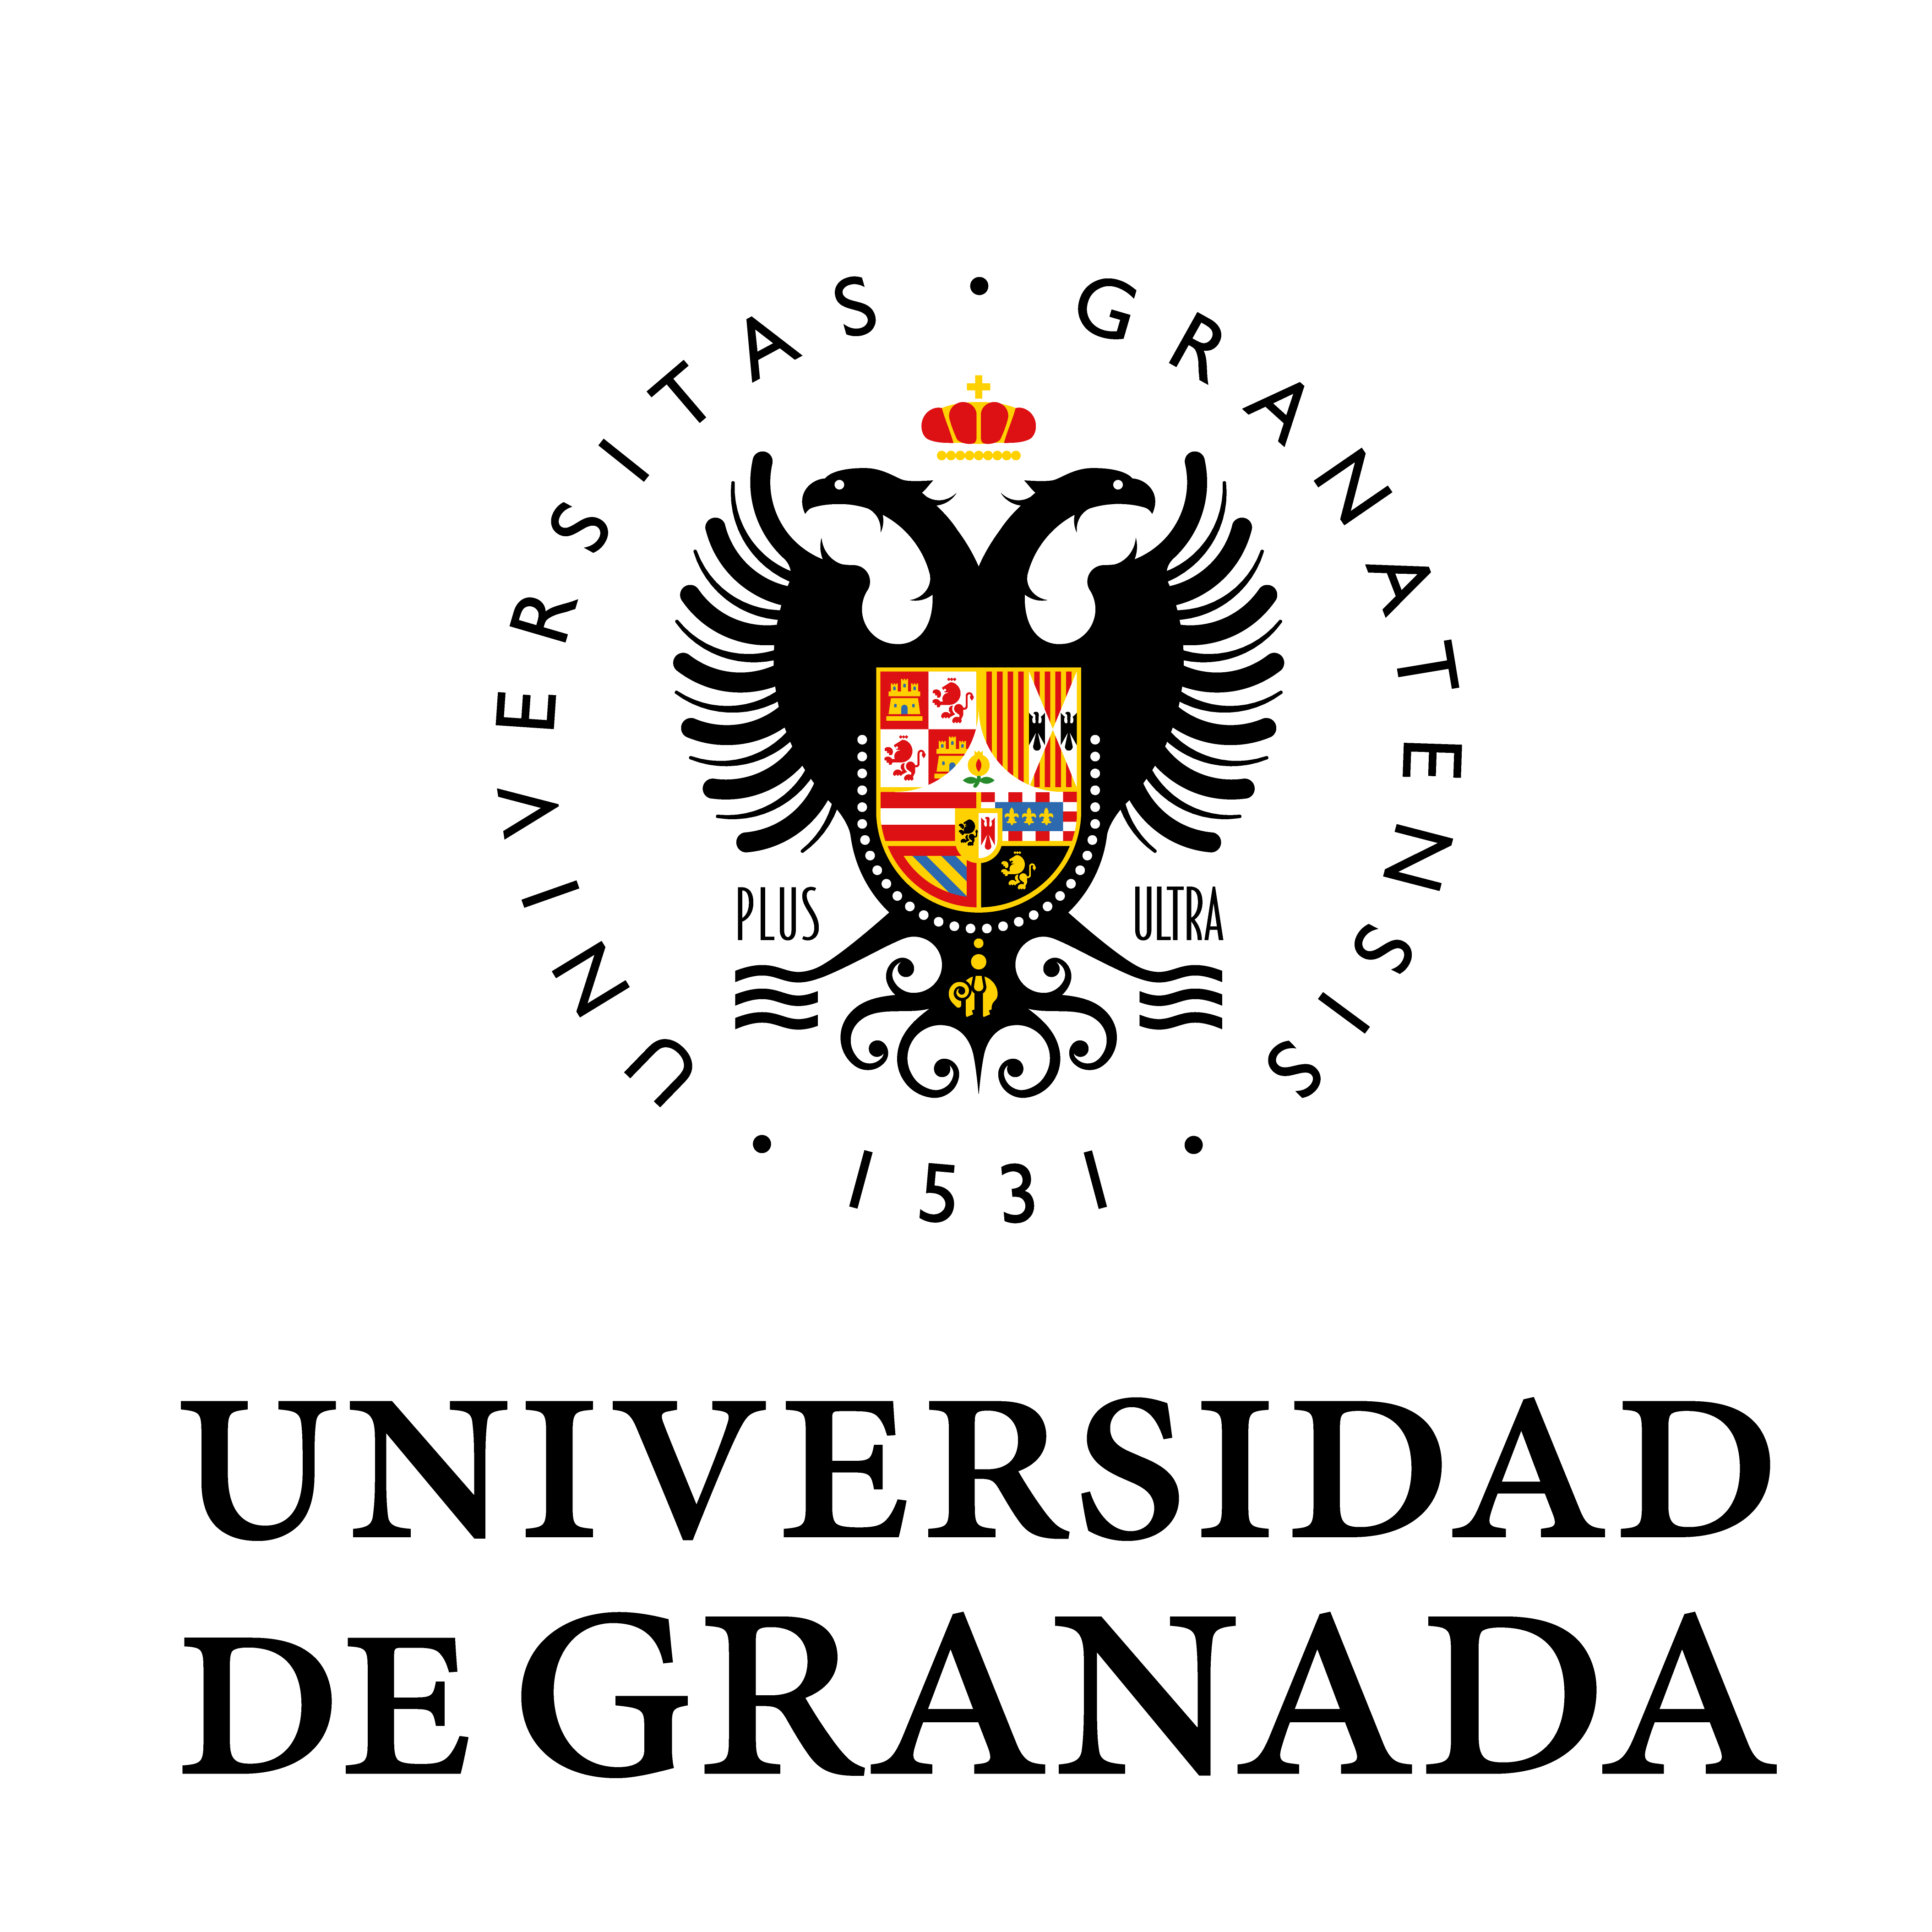
\includegraphics[scale=0.4]{img/logo_ugr.png}
\end{figure}

\begin{center}
  \Large TRABAJO FIN DE GRADO\\ 
  \large Doble grado en Ingeniería Informática y Matemáticas
  \vspace{0.7cm}

  \hrule
  \vspace{0.2cm}
  \textbf{\LARGE MW Store: facilitador genérico para proveedores de servicios con multi-inquilinato en una infraestructura Cloud}
  \vspace{0.2cm}
  \hrule
  \vspace{2cm}
  
  \textbf{Autor}

  Rubén Morales Pérez

  \vspace{2cm}
  \textbf{Director}

  Manuel Isidoro Capel Tuñón

  \textit{Departamento de Lenguajes y Sistemas Informáticos}
\end{center}

\newpage

\ 
\thispagestyle{empty}

\maketitle
\tableofcontents % Generando el indice
\setlength\parindent{0pt} % Quitamos la sangría

\newpage

\section{Introduction}
The influence of cloud computing and Software-as-a-Service (SaaS) is growing in enterprise software.
SaaS is frequently offered in a multi-tenant paradigm, where multiple customers (tenants) share resources such as software and hardware, without necessarily sharing data \cite{defining-multi-tenancy}.
Each tenant will be able to store the data for their own customers.
Multi-tenancy allows customization of the software according to the requirements of different customers.
Multi-tenancy is applicable to different levels in a system’s architecture and there are several architectural approaches to define it.
It's possible to refer to multi-tenancy using the whole picture of a system or increasing the granularity (i.e. database level).
Several core principles in multi-tenancy will be covered: data isolation, security, concurrent data access, scalability and performance.

\

\definition{NIST definition of cloud computing}{Cloud computing is a model for enabling convenient, on-demand network access to a shared pool of configurable computing resources (e.g., networks, servers, storage, applications, and services) that can be rapidly provisioned and released with minimal management effort or service provider interaction. \cite{cloud-computing-state-of-the-art}}

\

In general, cloud computing reduces business risks (such as hardware failures) and maintenance expenses by outsourcing the service infrastructure to the infrastructure providers \cite{cloud-computing-state-of-the-art}.
Virtualization allows cloud computing to pool computing resources from clusters of servers and distribute them dynamically to the applications.
Dynamic resource provisioning can be reactive to immediate demand fluctuations or proactive, allocating resources before they are needed using predicted demand \cite{cloud-computing-state-of-the-art}.
The architecture of cloud computing (Figure \ref{fig:cloud-computing-architecture}) can be described in four layers \cite{cloud-computing-state-of-the-art}:

\begin{itemize}
    \item Hardware layer: handle the physical resources of the cloud, servers, routers, switches, power and cooling systems.
    \item Infrastructure/virtualization layer: pool of storage and computing resources. Infrastructure as a Service (IaaS) refers to the on-demand provisioning of infrastructural resources like virtual machines.
    \item Platform layer: operating systems and application frameworks. It's main purpose is to minimize the effort to deploy applications on virtual machine containers. Platform as a Service (PaaS) refers to providing these resources on demand, examples of PaaS providers could be Google App Engine and Microsoft Windows Azure.
    \item Application layer: the actual cloud applications. Software as a Service (SaaS) provides on-demand applications over the Internet using web interfaces.
\end{itemize}

\begin{figure}[H]
  \centering
  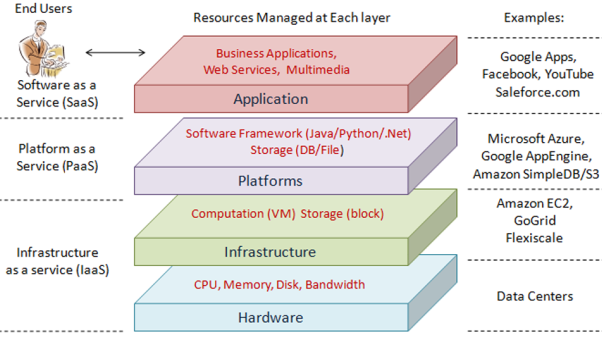
\includegraphics[scale=0.5]{img/cloud-computing-architecture.png}
  \caption{Cloud computing architecture \cite{cloud-computing-state-of-the-art}}
  \label{fig:cloud-computing-architecture}
\end{figure}

From an economic perspective, clouds are implemented in large data centers, achieving economy-of-scale and high manageability \cite{cloud-computing-state-of-the-art}.
The main drawbacks of this approach is the high energy expense and high initial investment.
On the other hand, small data centers does not consume so much power and are cheaper to build and can be distributed geographically easier than large data centers.

% TODO
% Software as a Service (SaaS) as an outsourcing model: An economic analysis
% https://www.researchgate.net/publication/228447677_Software_as_a_Service_SaaS_as_an_outsourcing_model_An_economic_analysis

% Cloud Computing-Software as Service 
% https://www.researchgate.net/publication/274481004_Cloud_Computing-Software_as_Service

\subsection{Classification}
% todo  SaaS Architecture Maturity Model


From the isolated approaches to more shared data \cite{multi-tenant-data-architecture}, multi-tenant data classification is an continuum:

\begin{itemize}
    \item Separate databases. It is the simplest approach to data isolation. Generally, computing resources and application code are shared between all the tenants, but data is logically separated. It adds an extra database data security layer, but it tends to higher costs, limiting the number of tenants to the number of databases that the server can support.
    \item Shared Database, Separate Schemas. Each tenant has its own set of tables grouped into a separated schema. This approach still allows for database permissions layer and it has lower costs that separate databases. It could be a good approach for applications with a small number of database tables.
    \item Shared Database, Shared Schema. Each table can include records from multiple tenants, a table column associates each record with the appropriate tenant. Data isolation is achieved through virtual isolation. This approach has the lowest hardware and backup costs, allowing the largest number of tenants per database server.
    \item Mixed approaches. It is possible to have separate databases/schemas for specific customer(s) and share schemas for other customers. This approach could fit the requirements of certain customers but the extra complexity must be justified.
\end{itemize}
\begin{figure}[ht]
  \centering
  
\includegraphics[scale=0.225]{img/multitenant-approaches.png}
\end{figure}
Some customers will have strongest data isolation requirements than others. Separate databases in practice would simply add an extra security layer due to more granularity regarding database access permissions. Some key points to decide which configuration is more appropriate for your business case are:
\begin{itemize}
    \item Number of tenants. The order of magnitude in number of tenants might prevent scalability with separate databases.
    \item Database size per tenant. Huge amounts of data per tenant would make shared approaches more inconvenient. Strategies like grouping tenants by geographical distribution could be considered to minimize this effect.
    \item Configurability, possibility of tailored tenant services. Separate databases would allow easier configurability per tenant, creating custom tables and columns in the database. The business model is relevant here because more shared approaches would make \href{https://en.wikipedia.org/wiki/Feature_toggle}{feature toggle} straight forward, allowing to turn on/off certain features on the fly.
\end{itemize}

\


On the other hand, just because a system is advertised as SaaS in the cloud does not mean it holds its benefits (savings, security, flexibility, disaster recovery, scalability, access to automatic updates, ...). % https://www.forbes.com/sites/forbesbusinesscouncil/2019/11/20/what-is-the-saas-architecture-maturity-model/
Microsoft describes an incremental SaaS maturity along three dimensions: configurability, multi-tenancy and scalability \cite{saas-maturity-model}. 
The axis of the maturity model combines the service component axis (core features of structuring software business) and the maturity levels (Figure \ref{fig:saas-maturity-model}):
\begin{itemize}
    \item Ad Hoc Level: dedicated database and schema without content sharing and multitenancy. It is handled with different applications on web interfaces for each user. With respect to the Service-level agreement (SLA), it depends on separated contracts reflecting the requirements for each user.
    \item Standardization Level: attempts to provide shared service. It shares the database using dedicated schema with configurable single tenants, allowing users to build their service model.
    \item Integration Level: multi tenant environment with shared database and schema. There is a predefined shared instance and configurable options for each tenant. The business layer focuses on measurable SLA adaptations.
    \item Virtualization Level: focus on scalability and availability.
    The data layer uses distributed computing.
    The virtualized system uses load-balancing across several service modules.
    User requirements are handled in the business process (instead of code customizations) and optimized SLA policies by measuring the amount of service used per customer
\end{itemize} 

\begin{figure}[H]
  \centering
  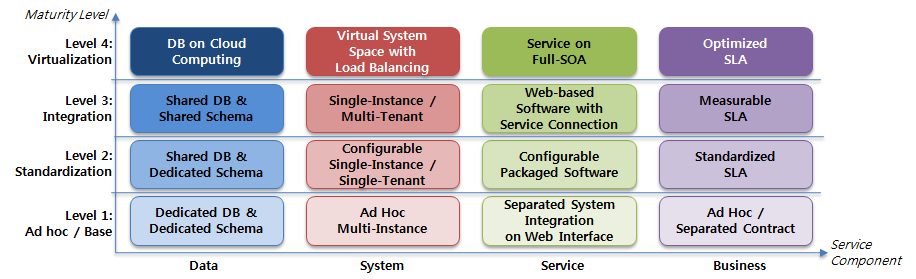
\includegraphics[scale=0.5]{img/saas-maturity-model.png}
  \caption{SaaS Maturity Model \cite{saas-maturity-model}}
  \label{fig:saas-maturity-model}
\end{figure}

The layered architecture of cloud computing allows a PaaS provider to run on top of an IaaS provider.
In practice, IaaS and PaaS belong to the same organization and are often called the infrastructure providers or cloud providers\cite{cloud-computing-state-of-the-art}.

\

Some service providers optimize operation costs, while others prefer high reliability and security.
There are several types of clouds available:
\begin{itemize}
    \item Public clouds: offering resources to the general public.
    \item Private clouds (internal clouds): exclusive for a given organization. They offer more control over performance, reliability and security at a higher cost than public clouds.
    \item Hybrid clouds: a combination of public and private clouds, the separation between public and private cloud components must be designed in advance.
    \item Virtual private clouds (VPC): a platform running on top of public clouds. It virtualizes servers, applications and the underlying communication network through virtual private networks.
\end{itemize}


\section{Security}
SaaS forces potential customers to partially shift control of their business data to a third party. Security is one the basic concerns that needs to be taken into account in order to gain customer trust. 
In risk analysis, multiple defense levels against both internal and external potential threats will increase the overall security. The system is only as strong as the weakest link in the chain.

\

SaaS applications provide an extra layer of security allowing to handle security in the back end, although extra layers of defense in the front end are a nice to have.
In desktop applications the code could potentially be reverse-engineering and modified to meet certain goals. % Citation needed
Security in the front end is a nice to have but we must take into account that any security layer implemented in the front end could potentially be bypassed.
% TODO: research about security in general SaaS applications

\

Security must be considered by design, not to rely on security through obscurity.
There are several security patterns (agnostic to the database management system) available for each data isolation approach \cite{multi-tenant-data-architecture}.
In the particular scenario of multi-tenancy, these security approaches should be taken into account to provide security at different levels:
\begin{itemize}
    \item Filtering: use an intermediary layer between a tenant and a data source, allowing access only to their tenant data (data isolation).
    In the code, this can be handled restricting the persistence layer access to certain database access objects filtering automatically the tenant data.
    Another safer possibility would be to use query interceptors to restrict database access to other tenants' data.
    The tenant id could be required for each request to the back end. For additional security, this tenant id can be stored in a temporal token previously generated and encrypted in the back end.
    \item Permissions: use access control lists (ACLs) to determine who (user and/or processes) can access data and what they can do with it. % TODO: research about ACLs
    Another desirable layer of security are enterprise virtual private networks that allows to restrict accesses to employees via Two-Factor Authentication.
    \item Encryption: obscuring every tenant's critical data so that it will remain inaccessible to unauthorized entities even with data leaks.
\end{itemize}

Certain security patterns can be used in all the possible scenarios (Separate Databases, Shared Database with Separate Schemas and Shared Database with Shared Schema)
\begin{itemize}
    \item Trusted Database Connections
    \item Secure Database Tables
    \item Tenant Data Encryption
\end{itemize}


\subsection{Trusted Database Connections}
Impersonation is one method to secure access to data stored in databases (Figure \ref{fig:impersonation-database-access}).
In this approach, the database is configured to allow individual users to access different tables, views, queries, stored procedures, and other database objects.
Any action that requires a call to the database use the user's security context to prevented undesired behaviour.
It's possible to create a database user for each tenant, restrict its access only to strictly required stuff and adapt the application to connect to the database on behalf of each user.

\

Another approach is the trusted subsystem access method (Figure \ref{fig:trusted-subsystem-database-access}).
In this scenario the application always connects to the database using its own application process identity.
Any additional security permission layer must be implemented within the application.
This approach is easier to handle, but it would not allow deeper permissions granularity.

\begin{figure}[h]
    \centering
    \begin{minipage}[t]{.5\textwidth}
      \centering
      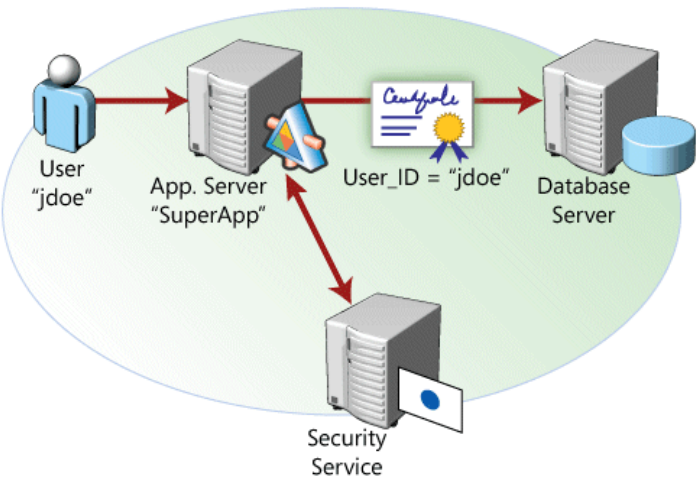
\includegraphics[width=0.75\linewidth]{img/impersonation-database-access.png}
      \caption{Impersonation database access
      \label{fig:impersonation-database-access}}
    \end{minipage}%
    \begin{minipage}[t]{.5\textwidth}
      \centering
      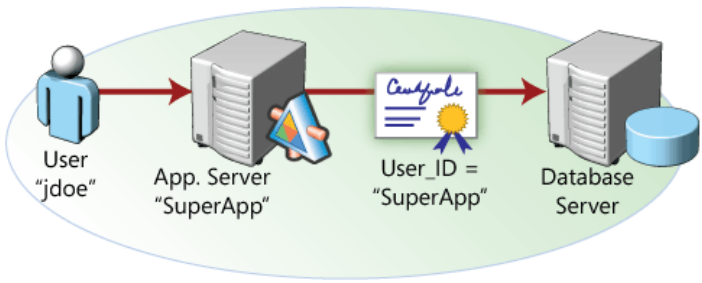
\includegraphics[width=1\linewidth]{img/trusted-subsystem-database-access.png}
      \caption{Trusted subsystem database access \label{fig:trusted-subsystem-database-access}}
    \end{minipage}
    % Image from multi-tenant-data-architecture cite
\end{figure}


\subsection{Secure Database Tables}
It's possible to secure a database with table granularity using the SQL GRANT command.
The following command will add the user account to the access control list for the table, allowing to restrict access only to a specific tenant user account:
\begin{lstlisting}[language=sql,numbers=none]
GRANT SELECT, UPDATE, INSERT, DELETE ON [TableName] FOR [UserName]
\end{lstlisting}

It's possible to restrict tenant access to their rows creating views, adding an extra layer of data isolation in shared schema approaches.
A view is a virtual table defined by the results of a SELECT query.
If there is a table called \textit{Table} and several tenants \{Tenant1, ..., TenantN\} it's possible to prevent direct read access to \textit{Table} and create several views \{Tenant1TableView, ..., TenantNTableView\}.
Each TenantXTableView will be the result of a SELECT query filtering with the tenant id column.

\begin{lstlisting}[language=sql,numbers=none]
CREATE VIEW Tenant1TableView AS
SELECT * FROM Table WHERE TenantID = SUSER_SID()
\end{lstlisting}

This statement obtains the security identifier (SID) of the tenant user account accessing the database.
In general, the tenant id is different to the tenant's SID so an extra table linking them could be needed (directly using the tenant id as filter would be less secure).
It's important to highlight that only read access could be restricted using this approach because the tenants still need to insert and update rows in the original table \textit{Table}.

\ 

Malicious/mistaken UPDATE, INSERT, DELETE statements from unauthorized tenant accounts could also be prevented in shared tables. It could be done using a similar approach with SID creating triggers (shown in Figure \ref{fig:tenant-triggers-data-isolation})

\begin{figure}[h]
\centering
\begin{minipage}[t]{.31\textwidth}
\centering
\begin{lstlisting}[language=sql,numbers=none]
DELIMITER $$

CREATE TRIGGER TENANT_PREVENT_INSERT
    BEFORE INSERT
    ON Table FOR EACH ROW
BEGIN
  IF NEW.TenantID != SUSER_SID() THEN  
    -- Throw error
  END IF;
END$$    

DELIMITER ;
\end{lstlisting}
\end{minipage}%
\hspace{0.3cm}
\begin{minipage}[t]{.31\textwidth}
\centering
\begin{lstlisting}[language=sql,numbers=none]
DELIMITER $$

CREATE TRIGGER TENANT_PREVENT_UPDATE
    BEFORE UPDATE
    ON Table FOR EACH ROW
BEGIN
  IF OLD.TenantID != SUSER_SID() THEN  
    -- Throw error
  END IF;
END$$    

DELIMITER ;
\end{lstlisting}
\end{minipage}
\hspace{0.3cm}
\begin{minipage}[t]{.31\textwidth}
\centering
\begin{lstlisting}[language=sql,numbers=none]
DELIMITER $$

CREATE TRIGGER TENANT_PREVENT_DELETE
    BEFORE DELETE
    ON Table FOR EACH ROW
BEGIN
  IF OLD.TenantID != SUSER_SID() THEN  
    -- Throw error
  END IF;
END$$    

DELIMITER ;
\end{lstlisting}
\end{minipage}
\caption{MySQL base trigger examples to prevent insert/update/delete different tenant data}
\label{fig:tenant-triggers-data-isolation}
\end{figure}


\subsection{Tenant Data Encryption}
Another security layer is database data encryption.
Cryptography can be categorized as either 
\begin{itemize}
    \item Symmetric: a key is generated to encrypt and decrypt data.
    \item Asymmetric (public‐key cryptography): two keys are generated, the public key is used to encrypt and the private key to decrypt.
\end{itemize}

Public‐key cryptography requires significantly more computing power than symmetric cryptography.
Encryption is a well-known technique, in multitenancy is possible to add an extra layer of security by creating different keys for each tenant.

% TODO? Guo C et al (2008) DCell: a scalable and fault-tolerant network structure for data centers. In: Proc SIGCOMM


\section{Extensibility}
Extensibility measures the ability and effort required to expand a system's behaviour.
It's a convenient pattern in the case of evolving systems which can not be designed entirely in advance.
Extensions of system's functionality increase the complexity and could make software maintainability harder. % TODO: citation needed
Just because it's possible to extend the software functionality doesn't mean we should.
An extensible design provides a framework to allow changes \cite{philosophy-extensible-software}, small increments will improve software reusability.

\

Traditional software development requirements will be needed for appropriate extensibility \cite{philosophy-extensible-software}:
\begin{itemize}
    \item High cohesion: degree to which part of the code forms a logically single and atomic unit. Example: classes that contain strongly related functionalities help to keep related parts of a codebase in a single place. % https://www.educative.io/edpresso/definition-high-cohesion
    % TODO: describe types of cohesion
    \item Low coupling: degree of interdependence between software modules. % https://en.wikipedia.org/wiki/Coupling_(computer_programming)
    Changes in more independent modules will not heavily impact other modules. % https://medium.com/clarityhub/low-coupling-high-cohesion-3610e35ac4a6
    \item Interface-implementation separation: allows you to change the implementation independently of the interface. 
    The use of polymorphism allow several implementations of the same interface in order to do similar things in different ways. % https://softwareengineering.stackexchange.com/questions/142192/why-would-a-programmer-want-to-separate-implementation-from-interface
    \item Dependencies: external dependencies are often needed to perform specific tasks. When a system grows is usually divided into several components, there will be internal inter-dependencies.
    \begin{figure}[H]
        \centering
        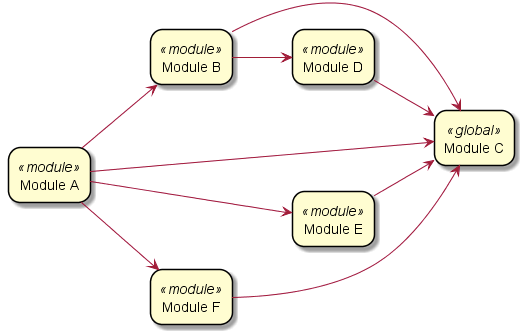
\includegraphics[scale=0.45]{img/dependency-graph.png}
        % https://github-wiki-see.page/m/devonfw/devon4node/wiki/guides-dependency-injection
        \label{fig:dependency-graph}
        \caption{Dependency graph}
    \end{figure}
    It's possible to automatically generate the dependency graph in order to inspect coupling or dangling dependencies (Figure \ref{fig:dependency-graph}). External dependencies tracking allows for the recognition of possible migrations to avoid non-maintained or vulnerable dependencies.
    Extensibility would lead to fewer and cleaner dependencies and well-defined interfaces \cite{philosophy-extensible-software}.
    \item Procedures to perform continuous integration: automate the integration of code changes from multiple contributors into a software project.
    Usage of automated tools for build, test and code analysis will allow faster feedback on new code’s correctness \cite{what-is-continuous-integration}.
    
    \
    
    Continuous Integration (CI) is generally used alongside an agile software development workflow \cite{what-is-continuous-integration}. 
    The next step is Continuous Delivery, responsible for packaging an artifact together ensuring that software is always ready to be delivered \cite{what-is-continuous-integration}.
    Continuous deployment is the final phase of the pipeline. The deployment phase is responsible for automatically launching and distributing the software artifact to end-users, automatically pushing code out when tests pass \cite{what-is-continuous-integration}.
\end{itemize}

% TODO: maximizing extensibility by means of design principles
% https://gupea.ub.gu.se/bitstream/handle/2077/20561/gupea_2077_20561_1.pdf;jsessionid=B2EA963686F0191DEED06BD96E805F6F?sequence=1

\

The extensible design fits well with Agile methodologies and iterative development, allowing re-prioritisation \cite{philosophy-extensible-software} looking at software as a growing entity.

% TODO: research about multi-module systems (Macroservices vs. Microservices) & CAP theorem linking it with software extensibility


\subsection{Multitenancy customization}
It's possible to conditionally extend a tenant functionality by addition of new features or through modification of existing ones.
There will be a set of tables/columns at the core of the application, but custom customer needs are not always addressable with a rigid data model.

\

There are three main ways to extend the data model to handle custom functionality \cite{multi-tenant-data-architecture}:
\begin{itemize}
    \item Preallocated Fields
    \item Name‐Value Pairs
    \item Custom columns
\end{itemize}

\

The data model can be customized creating custom fields in certain table(s) to allow tenants to extend their functionality \cite{multi-tenant-data-architecture} (Figure \ref{fig:preallocated-database-fields}).
This black box approach allows to determine how to use these fields depending on each customer, hiding actual data model complexity.
Nullable strings could be used as a flexible data type for the custom fields, avoiding unnecessarily data type restrictions (castings can be done in the code).

\begin{figure}[H]
    \centering
    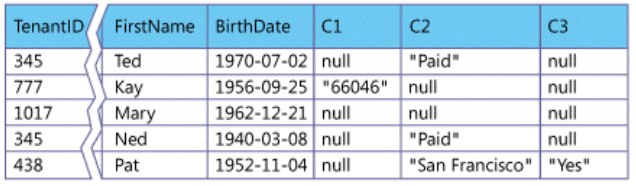
\includegraphics[scale=0.5]{img/preallocated-fields.png}
    \caption{Database table with preallocated fields C1, C2 and C3}
    \label{fig:preallocated-database-fields}
    % Cite multi-tenant-data-architecture
    % TODO generate figure with https://dbdiagram.io/d for uniform style
\end{figure}

\

Too few custom fields restrict tenants' customizability.
Too many custom fields will lead to a sparse database with many unused fields.
Name‐Value pairs allow each tenant to define an arbitrary number of custom fields \cite{multi-tenant-data-architecture} using one to many relationships with an external table (Figure \ref{fig:name-value-pairs-database}).
When the application retrieves a record from \textit{original\_table}, it performs a lookup in the extension table \textit{name\_value\_table}, selects all name-value pairs corresponding to the record id.
It's a good approach when specific customers require considerable flexibility and the shared database approach is used. 
The disadvantages of name-value approach are:
\begin{itemize}
    \item Extra complexity for database functions (such as indexing, querying, and updating records) 
    \item Black box approach with hidden types and possible database relationships
    \item Possible anti-pattern in the code
\begin{lstlisting}[language=python,numbers=none]
if isTenant1():
...
elif isTenant2():
...
\end{lstlisting}
\end{itemize}

\begin{figure}[H]
    \centering
    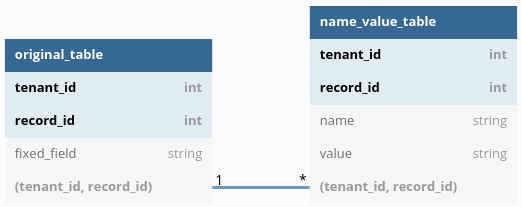
\includegraphics[scale=0.5]{img/name-value-pairs.png}
    \caption{Tenants custom fields using name-value pairs}
    \label{fig:name-value-pairs-database}
    % Cite multi-tenant-data-architecture
\end{figure}

\begin{comment}
% Source code to generate schema in https://dbdiagram.io/d
Table original_table {
  tenant_id int [pk]
  record_id int [pk]
  fixed_field string
}

Table name_value_table {
  tenant_id int [pk]
  record_id int [pk]
  name string
  value string
}

Ref: name_value_table.(tenant_id, record_id) > original_table.(tenant_id, record_id)
\end{comment}

\

Another extensible data model pattern is adding tailored columns to tenants' tables (Figure \ref{fig:custom-database-columns}).
This pattern is appropriate mostly for separate‐database or separate‐schema applications.
There would be extra  unneeded fields for several customers in a shared database environment when different tenants have radically different requirements.

\begin{figure}[H]
    \centering
    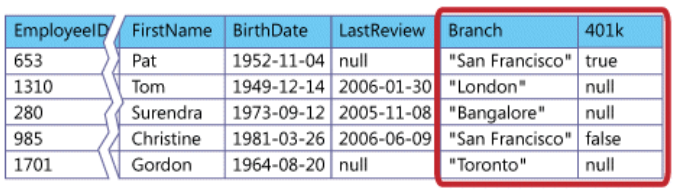
\includegraphics[scale=0.5]{img/custom-database-columns.png}
    \caption{Custom database columns extensibility approach}
    \label{fig:custom-database-columns}
    % Cite multi-tenant-data-architecture
\end{figure}

\   

Regardless of the extensibility pattern(s), any custom field will require a modification to the business logic, the presentation logic, or both.


% TODO: Configurability in SaaS (Software as a Service) Applications
% https://sci-hub.hkvisa.net/10.1145/1506216.1506221

\subsection{SaaS architecture approaches}
% TODO

\subsection{Deployments}
% TODO

\subsection{Software regressions}
A software regression is a special type of bug where a certain feature was working before and stops working.
Regressions can be produced due to changes in the code or the environment (i.e. system upgrades, environment variables, ...).
Regressions can be classified in:
\begin{itemize}
    \item Functional: a feature that is no longer working
    \item Performance: a feature is still working but more slowly or uses more resources (i.e. memory) than before
\end{itemize}

Testing can reduce regressions likelihood, and tests are either manual (sometimes involving Quality Assurance positions) or automatic.

\subsubsection{Automatic testing}
Automatic tests will catch bugs before production release and several strategies that can be used together:
\begin{itemize}
	\item End to end tests (E2E): involves entire workflows, typically front end, back end and database(s).
	\item Integration tests: specific use cases involving several components of a system.
	\item Unit tests: test cases involving only one component, mocking other components when needed. For example: in the back end, the database calls are not involved (just mocked), making the tests much faster.
\end{itemize}

The most convenient relationships between the number of tests for each strategy are described in the test pyramid:
\begin{figure}[H]
  \centering
  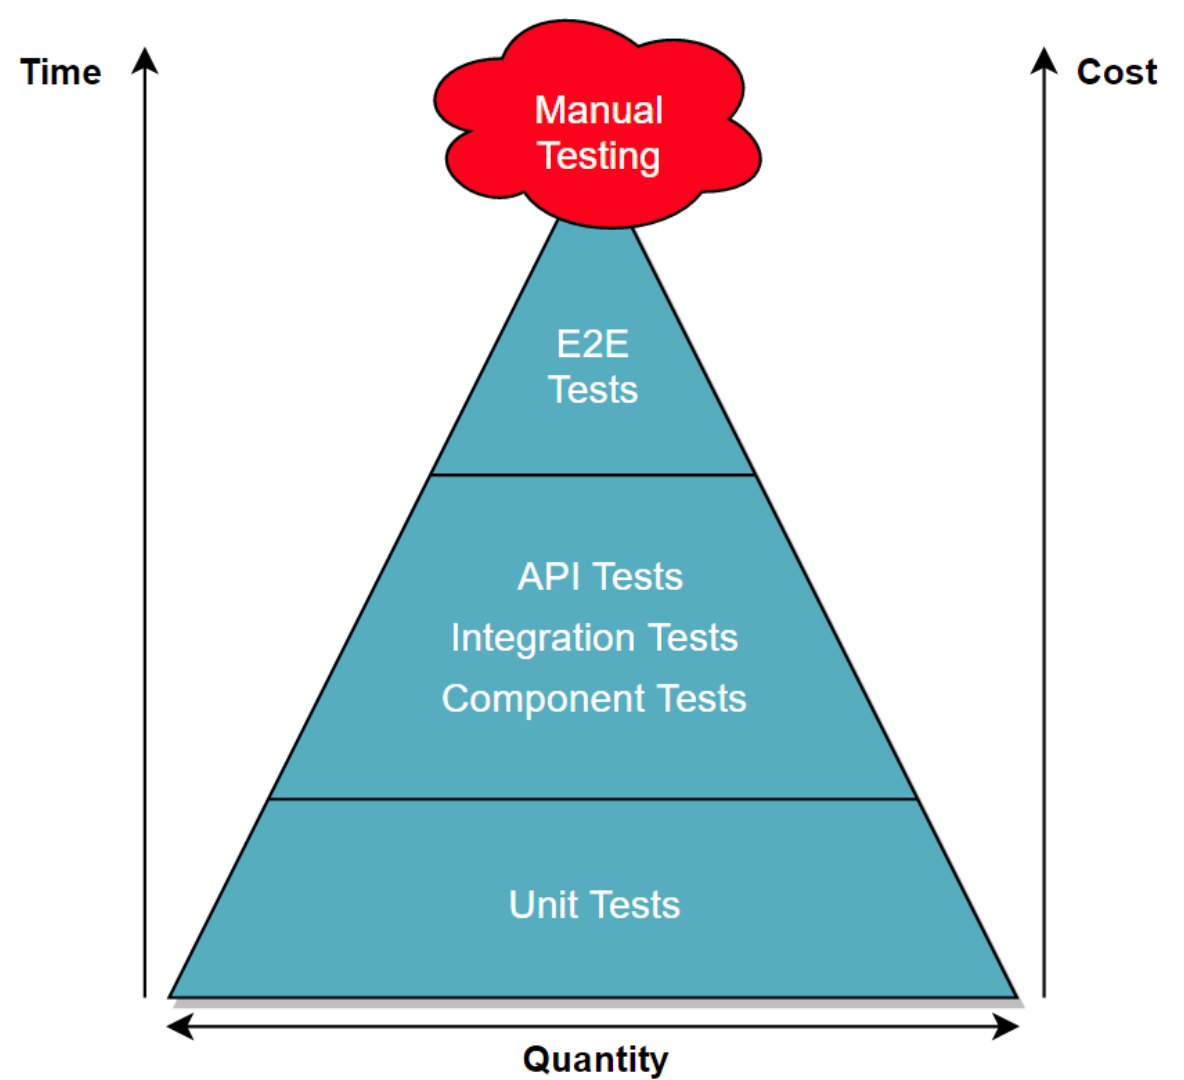
\includegraphics[scale=0.2]{img/test-pyramid.png}
  \caption{Test pyramid \cite{test-pyramid}}
\end{figure}

The inverted testing pyramid (fewer unit and integration tests, with an emphasis on automated and manual functional testing) is considered an anti-pattern, reducing the responsiveness, maintainability and reliability of the test setup \cite{test-pyramid}. 
Unit tests help identify faults in earlier phases \cite{test-pyramid} and must be the backbone of any software product.

\

Regression testing validates that the modified parts of a program do not introduce unexpected errors \cite{an-overview-of-regression-testing}.
Unit tests can be introduced in the continuous integration loop because their feedback is almost instantly
End to end and integration tests do not scale well % TODO: Citation needed
so it's not always possible to include all of them in the continuous integration loop.
Regression test selection techniques reduce the cost by selecting only the test cases related to a modified program (i.e. two consecutive commits in a version control system) \cite{regression-test-selection}.

\

There are other types of tests that should be considered:
\begin{itemize}
	\item Performance tests: check the system when it is under significant load, they are quite costly to implement and run. % https://www.atlassian.com/continuous-delivery/software-testing/types-of-software-testing
	\item Smoke tests: check basic functionality of the application. % https://www.atlassian.com/continuous-delivery/software-testing/types-of-software-testing
	\item Security Testing: check how the system reacts to internal and/or external threats (i.e. penetration testing). % https://www.softwaretestinghelp.com/types-of-software-testing/#1_Security_Testing
	\item Mutation tests: the code of a program is changed and verifies whether the existing test cases can identify these defects. It's a way to tests your tests, weak tests can produce a false sense of safety. % https://www.softwaretestinghelp.com/types-of-software-testing/#1_Security_Testing
\end{itemize}

\subsubsection{Tests detection}
% TODO

\subsection{Observability and monitoring}
Observability has its roots in control theory, addressing how to infer the internal state of a system by looking at its output. % https://www.thundra.io/hubfs/WP-%20Monitoring%20vs%20Observability/WP-MO.pdf

% TODO 
% https://www.thundra.io/hubfs/WP-%20Monitoring%20vs%20Observability/WP-MO.pdf
% From Observability to Significance in Distributed Information Systems
% On Observability and Monitoring of Distributed Systems: An Industry Interview Study


\section{Performance}
Large‐scale enterprise software is meant to be used by thousands of people simultaneously.
Performance is relevant in multi-tenant applications where a bottleneck affecting one customer could potentially affect several customers.
We need to distinguish between data scaling (increased capacity for storing and handling data) and application scaling (total workload that the application can handle) \cite{multi-tenant-data-architecture}.

% TODO: horizontal vs vertical scaling in applications


\subsection{Database}
Databases can be scaled up increasing server resources (more powerful processors, more memory, quicker disk drives, ...) and scaled out (partitioning one database onto multiple servers) \cite{multi-tenant-data-architecture}.

\subsection{Data scalability patterns}
There are two main tools to scale out a database:

\begin{itemize}
    \item Replication: copy all or part of a database to another spot(s), and then keep synchronized the copy (or copies) with the original. 
    If only the original database can be written to is called single-master replication. When it's possible to write into several copies of the database is called multi-master replication and requires a more complex synchronization mechanism to integrate the changes between the different copies.
    It's a good approach to create read‐only copies of data that doesn't change very often.
    \item Partitioning: subsets of the database are moved to other locations/databases.
    In horizontal partitioning, a table is divided into several databases using the same structure, resulting in tables with fewer rows.
    In vertical partitioning, a table is divided into smaller tables with the same number of rows but splitting the columns from the original table.
    This technique is useful when a monolithic application is splitted into several modules. Splitting the tables in a schema into several subsets allows for independently deployable modules.
    As a rule of thumb, try to find divisions in the data minimizing the number of cross‐database communications.
\end{itemize}

It's possible to create horizontal partitioning in a shared database based on tenant ids.
Different tenants can have very different demands.
It's necessary to prevent overtaxed partitions while other partitions are underused, i.e. partition the database to equalize the total number of active end users on each database.


\subsubsection{Concurrent data accesses}
% TODO: https://www.researchgate.net/publication/256481956_Teaching_concurrency_aspects_in_database_systems_in_a_practical_way
% https://www.cs.purdue.edu/homes/bb/cs542-06Spr-bb/cc.pdf
% https://fauna.com/blog/introduction-to-transaction-isolation-levels
% https://developpaper.com/transaction-management-in-relational-databases-concurrency-control-and-transaction-log/


\subsection{Cache}
\subsection{Quality of Service in Cloud Computing}
% TODO: Quality of Service in Cloud Computing Environments with Multi-tenant DBMS



\section{Petri nets}
A Petri net is a directed graph with two kinds of nodes,
interpreted as places and transitions,
such that no arc connects two nodes of the same kind.


\subsection{Concurrent systems validation}
% TODO Coloured Petri Nets





\section{Use case: e-commerce platform}
The system will store products (each product belonging to a specific tenant) and will allow normal users to order them. Each tenant could be an individual or organization and it will have a back office available to customize their product(s) and keep track of the orders.

\

Technological stack of the system:
\begin{itemize}
    \item Front end: Angular (testing with Karma + Jasmine)
    \item Back end: Java 11 (testing with JUnit)
    \item Database: MySQL (with agnostic database calls)
    % \item Continuous integration and delivery: Jenkins
    \item End to end tests: Selenium
    \item Code analysis: SonarQube
\end{itemize}


\subsection{Coverability Trees using Petri Nets}
\subsubsection{Availability}
\subsubsection{Vivacity?}
\subsubsection{Security}


\newpage
\printbibliography

\end{document}
